\chapter{Implementation and Side-Channel Resistance}
\label{ch:implementation}

\abstract*{Mathematical security is necessary but not sufficient: more cryptographic deployments are compromised through implementation flaws than through mathematical breakthroughs. This chapter addresses the engineering challenges of post-quantum cryptography, from constant-time programming and side-channel resistance to random number generation and the bandwidth implications of larger keys and ciphertexts.}

\abstract{Mathematical security is necessary but not sufficient: more cryptographic deployments are compromised through implementation flaws than through mathematical breakthroughs. This chapter addresses the engineering challenges of post-quantum cryptography, from constant-time programming and side-channel resistance to random number generation and the bandwidth implications of larger keys and ciphertexts.}

% =============================================================
% Adapted from notes.tex §5.1 (lines 6426–6943).
% New material: masking for NTT, fault injection, CMVP/FIPS 140-3.
% =============================================================


\section{The Constant-Time Imperative}
\label{sec:constant-time}

A cryptographic algorithm may be provably secure in the mathematical model, yet a careless implementation can leak the entire secret key through execution time alone.  Timing side channels\index{timing side channel} arise whenever the duration of a computation depends on secret data: a branch taken or not taken, a cache line hit or miss, a variable-latency instruction---any of these can reveal bits of the key to an attacker who measures wall-clock time over many executions~\cite{FIPS203}.

\subsection{Why Timing Variations Leak Secrets}
\label{subsec:timing-leak}

Consider an attacker who can query a decapsulation oracle and measure response time with nanosecond precision.  If the implementation contains a single conditional branch whose outcome depends on a secret coefficient, the attacker observes two clusters of timings.  By correlating timing with chosen ciphertexts, the attacker partitions the secret space and recovers coefficients one by one.  Kocher's seminal work showed that even \emph{average} timing differences of a few microseconds suffice when the attacker collects millions of measurements.

\begin{example}[A Timing Disaster: Barrett Reduction]
\label{ex:barrett-timing}
The Barrett reduction\index{Barrett reduction} computes $a \bmod q$ using multiplication by a precomputed factor instead of division.  A naive implementation finishes with a conditional correction:
\begin{lstlisting}[language=C]
// INSECURE: timing depends on secret value
int16_t barrett_reduce(int32_t a) {
    int32_t t = (a * BARRETT_FACTOR) >> BARRETT_SHIFT;
    t = a - t * KYBER_Q;
    if (t >= KYBER_Q) {   // SECRET-DEPENDENT BRANCH
        t -= KYBER_Q;
    }
    return (int16_t)t;
}
\end{lstlisting}
The branch on line~5 executes conditionally depending on~\texttt{t}, which correlates with the secret polynomial coefficient being reduced.  Over millions of NTT operations, the timing difference between the taken and not-taken paths leaks enough information to reconstruct the secret key.
\end{example}

The constant-time fix replaces the branch with an arithmetic mask:

\begin{lstlisting}[language=C]
// SECURE: constant-time Barrett reduction
int16_t barrett_reduce_ct(int32_t a) {
    int32_t t = (a * BARRETT_FACTOR) >> BARRETT_SHIFT;
    t = a - t * KYBER_Q;
    t -= KYBER_Q & ~((t - KYBER_Q) >> 31);  // branchless
    return (int16_t)t;
}
\end{lstlisting}

The expression \texttt{(t - KYBER\_Q) >> 31} produces an all-ones mask when $t < q$ and an all-zeros mask when $t \geq q$.  The subtraction is performed unconditionally; the mask selects whether the result is kept.

\subsection{Constant-Time Programming Patterns}
\label{subsec:ct-patterns}

The Barrett example illustrates a single instance of a pervasive problem.  Every arithmetic routine, every comparison, every loop that touches secret data must be scrutinised for variable-time behaviour.  The discipline reduces to four rules:

\begin{svgraybox}
\textbf{The four rules of constant-time programming.}
Every implementation that processes secret data must obey:
\begin{enumerate}
\item \textbf{No secret-dependent branches.}  All conditional logic on secret values must be replaced by arithmetic or bitwise select operations.
\item \textbf{No secret-dependent memory access patterns.}  Array indices derived from secret data cause cache-timing leaks; use constant-index sweeps with conditional moves.
\item \textbf{No variable-latency instructions on secret data.}  On many microarchitectures, integer division and floating-point operations have data-dependent latency.
\item \textbf{No early termination.}  Comparison routines must always examine every byte; loops must execute a fixed number of iterations.
\end{enumerate}
\end{svgraybox}

These rules apply to all three NIST standards.  ML-KEM~\cite{FIPS203} uses the Fujisaki--Okamoto transform, which requires a constant-time comparison of re-encrypted ciphertext.  ML-DSA~\cite{FIPS204} rejection-samples signatures in a loop that must always run a fixed number of iterations.  SLH-DSA~\cite{FIPS205} uses hash-based tree traversal with secret-dependent leaf selection that must be protected.

\subsection{Verification Tools}
\label{subsec:ct-tools}

Manual inspection is insufficient for verifying constant-time behaviour.  The following tools automate the analysis:

\begin{table}[t]
\caption{Constant-time verification tools}
\label{tab:ct-tools}
\begin{tabular}{p{2.5cm}p{3.5cm}p{5cm}}
\hline\noalign{\smallskip}
\textbf{Tool} & \textbf{Approach} & \textbf{Scope} \\
\noalign{\smallskip}\svhline\noalign{\smallskip}
\texttt{ctgrind}  & Valgrind-based taint tracking  & Detects branches and memory accesses on tainted (secret) data \\
\texttt{timecop}  & Valgrind memcheck extension     & Flags uninitialised-value-style errors for secret-dependent control flow \\
\texttt{dudect}   & Statistical black-box testing   & Measures timing distributions; no source access needed \\
\texttt{ct-verif} & LLVM-based formal verification  & Proves constant-time at the IR level \\
\noalign{\smallskip}\hline
\end{tabular}
\end{table}

For production code, a combination of static analysis (\texttt{ct-verif}) and dynamic testing (\texttt{dudect}) provides the strongest assurance.  Constant-time discipline eliminates timing as a side channel, but timing is not the only channel an attacker can exploit.  Power consumption, electromagnetic emanation, and cache behaviour all leak information---and lattice-based schemes introduce attack surfaces that have no classical analogue.


%% ================================================================
\section{Side Channels in Lattice Cryptography}
\label{sec:side-channels}

The NTT, polynomial sampling, and the Fujisaki--Okamoto decapsulation check each present distinct attack opportunities that deserve individual attention.

\subsection{Timing Attacks on the NTT}
\label{subsec:ntt-timing}

The NTT\index{NTT!side channel} is the performance-critical kernel of ML-KEM and ML-DSA: it reduces polynomial multiplication from $\bigO(n^2)$ to $\bigO(n \log n)$.  Each butterfly operation involves a modular multiplication followed by modular reduction.  If the reduction uses a conditional subtraction (as in \cref{ex:barrett-timing}), the attacker can correlate timing with individual coefficients of the secret polynomial.

A constant-time butterfly avoids all branches:

\begin{lstlisting}[language=C]
// Constant-time NTT butterfly with Montgomery reduction
void ct_butterfly(int16_t *a, int16_t *b, int16_t zeta) {
    int32_t t = (int32_t)montgomery_reduce((int32_t)*b * zeta);
    *b = *a - t;
    *a = *a + t;
    // Branchless conditional reduction
    *a -= KYBER_Q & -((*a >= KYBER_Q));
    *b += KYBER_Q & -((*b < 0));
}
\end{lstlisting}

\subsection{Power and Electromagnetic Analysis}
\label{subsec:power-em}

Timing attacks require only network access, but an attacker with physical proximity can extract far more.  Simple Power Analysis (SPA)\index{SPA} and Differential Power Analysis (DPA)\index{DPA} exploit the fact that different instructions and data values draw different amounts of current.  A single power trace of an NTT execution can reveal the structure of the butterfly network, and by extension the secret polynomial.

\textbf{SPA on lattice operations.}  The NTT butterfly has a characteristic power signature: the multiply-and-reduce step draws measurably more current than addition.  When the reduction step is conditional, the power trace directly reveals whether the subtraction occurred.  For ML-DSA, the rejection sampling loop produces a variable number of NTT calls per signature; the number of iterations visible in the power trace leaks information about the secret key.

\textbf{DPA on polynomial coefficients.}  By collecting thousands of power traces during decapsulation and correlating with hypothesised coefficient values, an attacker mounts a DPA attack that recovers the secret polynomial coefficient by coefficient.  The attack succeeds because each butterfly operation processes one coefficient against one twiddle factor, creating a localised power-secret dependency.

\textbf{Electromagnetic emanation attacks.}  EM probes placed near the processor die can achieve spatial resolution sufficient to isolate individual pipeline stages.  This is particularly threatening for embedded implementations (smart cards, IoT devices) where the attacker may have physical access.

\subsection{Cache-Timing Attacks}
\label{subsec:cache-timing}

Power and EM attacks require physical proximity, but cache-timing attacks can be mounted by any process sharing the same hardware---including a co-tenant in a cloud virtual machine.  Table-based implementations of modular arithmetic or hash functions are vulnerable to cache-timing attacks\index{cache-timing attack}.  When a lookup table exceeds one cache line (typically 64 bytes), the access pattern reveals which entries were used.  In lattice cryptography, this affects:

\begin{itemize}
\item \textbf{NTT twiddle factor tables.}  If the table of roots of unity is large enough to span multiple cache lines, the access pattern during the NTT reveals structural information about the transform.
\item \textbf{Discrete Gaussian sampling via CDT.}  The cumulative distribution table (CDT) method performs a binary search; the sequence of cache lines accessed reveals the sampled value.
\item \textbf{SHAKE/SHA-3 round functions.}  The Keccak permutation is naturally constant-time, but software implementations that use lookup tables for the $\chi$ step may leak.
\end{itemize}

The countermeasure is to ensure all table accesses sweep the entire table in constant time, selecting the desired entry via conditional moves.

Figure~\ref{fig:ch12-gaussian-sampling} summarises the security--efficiency tradeoff among the principal Gaussian sampling strategies: rejection sampling is simple but variable-time, CDT is fast but vulnerable to cache attacks, and inversion sampling achieves constant-time execution at the cost of additional implementation complexity.

\begin{figure}[t]
\centering
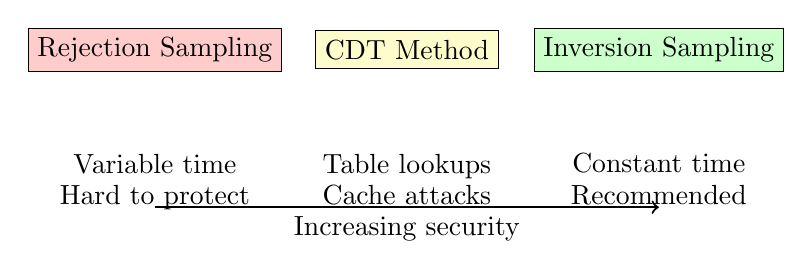
\begin{tikzpicture}[scale=0.8]
    % Gaussian sampling methods
    \node[draw, rectangle, fill=red!20] (rej) at (0,2) {Rejection Sampling};
    \node[draw, rectangle, fill=yellow!20] (cdt) at (4,2) {CDT Method};
    \node[draw, rectangle, fill=green!20] (inv) at (8,2) {Inversion Sampling};

    % Properties
    \node[below] at (0,0.5) {Variable time};
    \node[below] at (0,0) {Hard to protect};

    \node[below] at (4,0.5) {Table lookups};
    \node[below] at (4,0) {Cache attacks};

    \node[below] at (8,0.5) {Constant time};
    \node[below] at (8,0) {Recommended};

    % Arrows
    \draw[thick, ->] (0,-0.5) -- (8,-0.5);
    \node[below] at (4,-0.5) {Increasing security};
\end{tikzpicture}
\caption{Gaussian sampling methods and their side-channel tradeoffs.  Rejection sampling is variable-time and difficult to protect; CDT is fast but leaks through cache access patterns; inversion sampling achieves constant-time execution at the cost of greater implementation complexity.}
\label{fig:ch12-gaussian-sampling}
\end{figure}

\subsection{Masking Countermeasures for the NTT}
\label{subsec:masking-ntt}

Constant-time code defeats timing and cache attacks, but it cannot hide power consumption or electromagnetic emanation---the physics of computation guarantees that different data values draw different currents.  Masking\index{masking} is the standard countermeasure against power and EM analysis.  The idea is to split every secret value $x$ into $d+1$ shares $x_0, \ldots, x_d$ such that $x = x_0 + x_1 + \cdots + x_d \bmod q$, where each share is individually uniformly random.  An attacker who observes fewer than $d+1$ shares learns nothing about~$x$.

\begin{definition}[Boolean and Arithmetic Masking]
\label{def:masking}
Let $x \in \Zq$ be a secret value.
\begin{itemize}
\item \textbf{Boolean masking\index{masking!Boolean}:} choose $r \getsr \{0,1\}^k$ and store $(x \oplus r,\; r)$.
\item \textbf{Arithmetic masking\index{masking!arithmetic}:} choose $r \getsr \Zq$ and store $(x - r \bmod q,\; r)$.
\end{itemize}
A $d$-th order masking scheme uses $d+1$ shares and is secure against attackers who can probe at most $d$ intermediate values simultaneously.
\end{definition}

Applying masking to the NTT is non-trivial because the butterfly mixes shares through both addition and multiplication.  The state of the art proceeds as follows:

\begin{enumerate}
\item Mask all input coefficients with arithmetic shares before entering the NTT.
\item Perform the NTT independently on each share (the NTT is linear over $\Zq$, so $\mathrm{NTT}(x_0 + x_1) = \mathrm{NTT}(x_0) + \mathrm{NTT}(x_1)$).
\item For pointwise multiplication (which is non-linear), use a secure multiplication gadget that refreshes shares after every product.
\item Recombine shares only at the final output, after all secret-dependent operations are complete.
\end{enumerate}

The overhead of first-order masking ($d=1$) is roughly $2$--$3\times$ in execution time and $2\times$ in memory.  Higher-order masking scales as $\bigO(d^2)$ due to the secure multiplication gadget.

\begin{remark}[Masking vs.\ Hiding]
Masking (splitting secrets into shares) and hiding (adding random delays or shuffling operation order) are complementary.  Production implementations targeting smart-card certification (Common Criteria EAL4+ or higher) typically combine both.
\end{remark}

All the attacks discussed so far---timing, power, EM, cache---are \emph{passive}: the attacker observes but does not interfere.  A stronger adversary can actively corrupt a computation and exploit the faulty output.


%% ================================================================
\section{Fault Injection Attacks}
\label{sec:fault-injection}

Fault injection\index{fault injection} encompasses a family of techniques---voltage glitches, clock manipulation, laser pulses, electromagnetic pulses---that induce physical perturbations and exploit the resulting errors to recover secrets.  The attacker's toolkit ranges from inexpensive glitching hardware to precision laser stations costing hundreds of thousands of euros.

\subsection{Fault Models}
\label{subsec:fault-models}

The standard fault models, ordered by attacker strength, are:

\begin{enumerate}
\item \textbf{Instruction skip.}  A single instruction is replaced by a NOP.  This is achievable with voltage or clock glitches and requires only coarse temporal control.
\item \textbf{Random byte/word fault.}  A storage element (register or SRAM cell) is set to a random value.  Laser fault injection achieves this with spatial precision of a few micrometres.
\item \textbf{Bit flip.}  A single bit in a register or memory cell is toggled.  Focused ion beam or precise laser attacks can target individual bits.
\item \textbf{Stuck-at fault.}  A bit is forced to~0 or~1 permanently.  This models persistent hardware damage.
\end{enumerate}

\subsection{Attacks on ML-DSA (Dilithium)}
\label{subsec:fault-dilithium}

ML-DSA~\cite{FIPS204} uses rejection sampling: after computing a candidate signature $\mathbf{z} = \mathbf{y} + c\mathbf{s}_1$, the signer checks $\norm{\mathbf{z}}_\infty < \gamma_1 - \beta$.  If the check fails, the signer restarts with fresh randomness.

\textbf{Skipping the rejection check.}  If an attacker can induce an instruction skip that bypasses the norm check, the faulty signature is output without rejection.  This signature leaks information about $\mathbf{s}_1$: without the bound on $\norm{\mathbf{z}}_\infty$, the distribution of $\mathbf{z}$ is no longer independent of the secret.  Collecting a few hundred faulty signatures enables full key recovery via lattice reduction.

\textbf{Faulting the hash computation.}  If the challenge hash $c = H(\mu \| \mathbf{w}_1)$ is corrupted, the resulting signature $(c', \mathbf{z})$ satisfies $\mathbf{z} = \mathbf{y} + c'\mathbf{s}_1$ for a known $c'$.  Two signatures with the same $\mathbf{y}$ but different challenges yield $\mathbf{z}_1 - \mathbf{z}_2 = (c_1' - c_2')\mathbf{s}_1$, recovering $\mathbf{s}_1$ directly.

\subsection{Attacks on ML-KEM (Kyber)}
\label{subsec:fault-kyber}

ML-KEM~\cite{FIPS203} uses the Fujisaki--Okamoto (FO) transform, which re-encrypts the decrypted message and compares the result to the received ciphertext.  If they match, the shared secret is derived from the message; otherwise, an implicit rejection value is returned.

\textbf{Faulting the FO comparison.}  If the attacker skips the re-encryption check, the oracle always returns the ``real'' shared secret, converting the CCA-secure scheme into a CPA-only scheme.  The attacker then mounts a chosen-ciphertext attack against the underlying CPA encryption, recovering the secret key.

\textbf{Faulting decryption coefficients.}  A random fault during inverse-NTT corrupts a single coefficient of the decrypted polynomial.  By submitting the same ciphertext multiple times and comparing correct and faulted outputs, the attacker isolates individual coefficients of the secret key.

\subsection{Countermeasures}
\label{subsec:fault-countermeasures}

\begin{table}[t]
\caption{Fault injection countermeasures and their overhead}
\label{tab:fault-countermeasures}
\begin{tabular}{p{3cm}p{5cm}p{3cm}}
\hline\noalign{\smallskip}
\textbf{Countermeasure} & \textbf{Mechanism} & \textbf{Overhead} \\
\noalign{\smallskip}\svhline\noalign{\smallskip}
Redundant computation & Execute critical operations twice and compare results & $\sim\!2\times$ time \\
Algorithm-level checksums & Verify $\mathbf{A}\mathbf{s} + \mathbf{e} = \mathbf{t}$ after key generation & Low ($< 5\%$) \\
Instruction flow monitoring & Hardware watchdog or software control-flow integrity & $10$--$20\%$ \\
Infection countermeasure & Randomise output on detected fault (no error signal) & Negligible \\
\noalign{\smallskip}\hline
\end{tabular}
\end{table}

The most effective strategy combines algorithmic redundancy (recompute and compare) with randomised fault detection (infection).  An attacker who cannot distinguish a detected fault from a natural rejection gains no information.

\begin{remark}[The Physics of Fault Injection]
Laser fault injection uses focused infrared pulses ($\lambda \approx 1064\,\mathrm{nm}$) to generate photo-currents in SRAM cells, flipping bits with spatial resolution of $\sim\!1\,\mu\mathrm{m}$.  Electromagnetic fault injection (EMFI) uses a coil probe to induce transient currents, offering lower precision but no requirement for decapsulation of the chip package.  Both techniques are available as commercial test equipment for security evaluation laboratories.
\end{remark}

Side channels and fault attacks exploit the physical computation; a different class of vulnerability targets the inputs to that computation.  If the random numbers feeding key generation or signing are weak, no amount of constant-time discipline or masking can save the scheme.


%% ================================================================
\section{Random Number Generation}
\label{sec:rng}

Lattice-based cryptography is extraordinarily hungry for randomness.  ML-KEM key generation requires sampling an entire matrix $\mathbf{A} \in \Zq^{k \times k}$ of polynomials plus secret and error vectors---thousands of random coefficients per operation.  Poor randomness does not merely weaken security; it can destroy it completely.

\subsection{DRBG Requirements}
\label{subsec:drbg}

NIST SP~800-90A specifies three approved Deterministic Random Bit Generators (DRBGs)\index{DRBG}: \texttt{CTR\_DRBG} (based on AES), \texttt{Hash\_DRBG} (based on SHA-2), and \texttt{HMAC\_DRBG}.  All three NIST post-quantum standards use SHAKE-128 or SHAKE-256 (instances of SHA-3) to expand a seed into the required random bytes, effectively using the seed-expansion paradigm internally.

The critical requirement is the quality of the initial seed.  A DRBG seeded with 256~bits of true entropy provides $2^{256}$ security regardless of how many bytes are subsequently generated.  A DRBG seeded with 15~bits of entropy (as in the 2008 Debian OpenSSL disaster\index{Debian OpenSSL bug}) reduces the entire key space to $2^{15}$, and the lattice structure makes key recovery even easier than brute force: the error distribution collapses, and simple linear algebra suffices.

\subsection{Hardware and Quantum Random Number Generation}
\label{subsec:hw-qrng}

\textbf{Hardware RNG (HRNG).}  Modern processors include hardware entropy sources: Intel's \texttt{RDRAND}/\texttt{RDSEED} (thermal noise in a metastable circuit), ARM's \texttt{TRNG} (ring oscillator jitter).  These provide the seed entropy that DRBGs expand.  The Linux kernel's \texttt{getrandom()} system call blocks until sufficient entropy is available, making it the recommended interface.

\textbf{Quantum RNG (QRNG).}  Quantum random number generators\index{QRNG} exploit the fundamental indeterminacy of quantum measurements---typically photon arrival times, vacuum fluctuations, or beam splitter outcomes.  Unlike classical entropy sources, whose unpredictability rests on complexity assumptions, QRNG unpredictability is guaranteed by the laws of physics.  For post-quantum cryptography, there is a pleasing conceptual closure: the same quantum mechanics that threatens classical cryptography provides provably random seeds for its replacement.

Regardless of the entropy source, the raw output is \emph{uniform} random bits, whereas lattice-based schemes require samples drawn from a discrete Gaussian distribution.  Figure~\ref{fig:ch12-rng-transform} illustrates this fundamental transformation challenge: converting a flat uniform distribution into the bell-shaped Gaussian that the cryptographic scheme demands, without introducing timing leaks or statistical bias.

\begin{figure}[t]
\centering
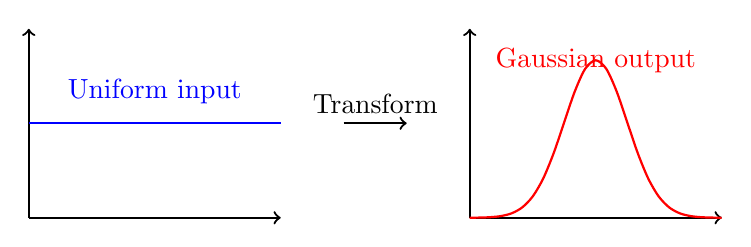
\begin{tikzpicture}[scale=0.8]
    % Uniform to Gaussian transformation
    \draw[thick, ->] (0,0) -- (0,3);
    \draw[thick, ->] (0,0) -- (4,0);
    \draw[thick, blue] (0,1.5) -- (4,1.5);
    \node[blue] at (2,2) {Uniform input};

    \draw[thick, ->] (5,1.5) -- (6,1.5);
    \node[above] at (5.5,1.5) {Transform};

    \draw[thick, ->] (7,0) -- (7,3);
    \draw[thick, ->] (7,0) -- (11,0);
    \draw[thick, red] plot[smooth, domain=7:11]
        (\x, {2.5*exp(-2*(\x-9)*(\x-9))});
    \node[red] at (9,2.5) {Gaussian output};
\end{tikzpicture}
\caption{The RNG transformation challenge: uniform random bits from the entropy source must be converted into a discrete Gaussian distribution required by lattice-based schemes, without introducing timing side channels or statistical bias.}
\label{fig:ch12-rng-transform}
\end{figure}

\subsection{Deterministic Key Generation}
\label{subsec:deterministic-keygen}

All three NIST standards support deterministic key generation from a single 32-byte seed:

\begin{lstlisting}[language=C]
// ML-KEM: deterministic key generation (FIPS 203, Algorithm 16)
void ml_kem_keygen(uint8_t *pk, uint8_t *sk, const uint8_t seed[32]) {
    uint8_t expanded[64];
    shake256(expanded, 64, seed, 32);
    // expanded[0..31] -> seed for matrix A
    // expanded[32..63] -> seed for secret/error
    expand_A(A, expanded);
    sample_secret(s, e, expanded + 32);
    pk = encode(A, A*s + e);
    sk = encode(s, pk, H(pk), z);  // z = implicit rejection seed
}
\end{lstlisting}

\textbf{Advantages:} reproducible key generation for testing, reduced RNG exposure surface (one call instead of many), and the ability to recover keys from a backed-up seed.

\textbf{Risks:} seed compromise is total compromise, and the seed expansion itself must be protected against side channels.

\begin{remark}[Hedged Randomness]
A prudent implementation \emph{hedges} by mixing the output of the system RNG with a deterministic component: $\text{seed} = H(\text{DRBG output} \| \text{nonce} \| \text{context})$.  If either source is compromised, the other provides a safety net.
\end{remark}

With constant-time code, side-channel countermeasures, fault resistance, and sound randomness in place, the implementation is secure---but it is also larger.  The next section quantifies the cost in bytes.


%% ================================================================
\section{Key and Ciphertext Sizes}
\label{sec:sizes}

The most immediate practical consequence of post-quantum cryptography is larger keys and ciphertexts.  Table~\ref{tab:pqc-sizes} presents a comprehensive comparison of all NIST post-quantum standards against classical baselines.

\begin{table}[t]
\caption{Key, signature, and ciphertext sizes for NIST PQC standards (bytes)}
\label{tab:pqc-sizes}
\begin{tabular}{p{3.2cm}rrrr}
\hline\noalign{\smallskip}
\textbf{Algorithm} & \textbf{Public key} & \textbf{Secret key} & \textbf{Sig./CT} & \textbf{Security} \\
\noalign{\smallskip}\svhline\noalign{\smallskip}
\multicolumn{5}{l}{\textit{Classical baselines}} \\
ECDH-P256         &   64 &   32 &   64\textsuperscript{CT} & 128-bit \\
Ed25519            &   32 &   32 &   64\textsuperscript{Sig} & 128-bit \\
RSA-3072           &  384 &  384 &  384\textsuperscript{Sig} & 128-bit \\
\noalign{\smallskip}\hline\noalign{\smallskip}
\multicolumn{5}{l}{\textit{ML-KEM (FIPS 203)---Key Encapsulation}} \\
ML-KEM-512         &  800 & 1{,}632 &  768\textsuperscript{CT} & 128-bit \\
ML-KEM-768         & 1{,}184 & 2{,}400 & 1{,}088\textsuperscript{CT} & 192-bit \\
ML-KEM-1024        & 1{,}568 & 3{,}168 & 1{,}568\textsuperscript{CT} & 256-bit \\
\noalign{\smallskip}\hline\noalign{\smallskip}
\multicolumn{5}{l}{\textit{ML-DSA (FIPS 204)---Digital Signature}} \\
ML-DSA-44          & 1{,}312 & 2{,}560 & 2{,}420\textsuperscript{Sig} & 128-bit \\
ML-DSA-65          & 1{,}952 & 4{,}032 & 3{,}309\textsuperscript{Sig} & 192-bit \\
ML-DSA-87          & 2{,}592 & 4{,}896 & 4{,}627\textsuperscript{Sig} & 256-bit \\
\noalign{\smallskip}\hline\noalign{\smallskip}
\multicolumn{5}{l}{\textit{SLH-DSA (FIPS 205)---Hash-Based Signature}} \\
SLH-DSA-128s       &   32 &   64 & 7{,}856\textsuperscript{Sig} & 128-bit \\
SLH-DSA-128f       &   32 &   64 & 17{,}088\textsuperscript{Sig} & 128-bit \\
SLH-DSA-192s       &   48 &   96 & 16{,}224\textsuperscript{Sig} & 192-bit \\
SLH-DSA-256s       &   64 &  128 & 29{,}792\textsuperscript{Sig} & 256-bit \\
\noalign{\smallskip}\hline
\end{tabular}
\end{table}

\subsection{Impact on TLS}
\label{subsec:tls-impact}

A TLS~1.3 handshake with X25519~+~Ed25519 transmits approximately 1.5\,KB of cryptographic material (key shares, certificates, signatures).  Replacing this with ML-KEM-768~+~ML-DSA-65 increases the cryptographic payload to roughly 9\,KB---a $6\times$ increase.  With a typical certificate chain of three certificates, the total signature contribution alone is $3 \times 3{,}309 = 9{,}927$~bytes, requiring TCP fragmentation and potentially an additional round trip.

\begin{example}[Handshake Overhead Calculation]
\label{ex:tls-overhead}
Consider replacing X25519 (32\,B public key) + Ed25519 (32\,B public key, 64\,B signature) with ML-KEM-768 + ML-DSA-65 in a TLS~1.3 handshake:
\begin{itemize}
\item Key exchange overhead: $(1{,}184 + 1{,}088) - (32 + 32) = +2{,}208$\,B.
\item Authentication overhead (3-cert chain): $3 \times (1{,}952 + 3{,}309) - 3 \times (32 + 64) = +15{,}495$\,B.
\item Total additional bytes: $\approx 17{,}700$\,B.
\end{itemize}
With a 1{,}500-byte MTU, the classical handshake fits in $\sim\!2$ TCP segments; the post-quantum handshake requires $\sim\!14$ segments and may need an additional round trip.
\end{example}

\subsection{Storage and Compression}
\label{subsec:storage}

\textbf{Certificate databases.}  A certificate authority storing $10^6$ end-entity certificates sees public-key storage grow from 32\,MB (Ed25519) to 1.95\,GB (ML-DSA-65)---a $61\times$ increase that has infrastructure implications for database indexing, replication, and backup.

\textbf{Blockchain.}  A Bitcoin transaction is approximately 250~bytes; replacing ECDSA with ML-DSA-65 would increase this to $\sim\!3{,}500$~bytes, accelerating blockchain growth by $14\times$.

\textbf{Compression techniques.}  Lattice public keys exhibit algebraic structure that enables moderate compression:
\begin{itemize}
\item \textbf{Seed expansion.}  Store only the 32-byte seed for the matrix $\mathbf{A}$ and transmit $\mathbf{t} = \mathbf{A}\mathbf{s} + \mathbf{e}$; the receiver re-expands $\mathbf{A}$ from the seed.  This is already standard in ML-KEM and ML-DSA.
\item \textbf{Coefficient compression.}  ML-KEM compresses ciphertext coefficients from 12~bits to 10 or 4~bits (depending on the component), reducing ciphertext size by $\sim\!25\%$ at the cost of a small decryption failure probability.
\item \textbf{Hybrid schemes.}  During the transition period, using a compact classical algorithm alongside PQC (e.g., X25519~+~ML-KEM-768) adds only $\sim\!32$~bytes over the PQC-only cost while providing backward security.
\end{itemize}

Larger artefacts demand more bandwidth, but how much \emph{time} do they cost?  Byte counts alone do not answer the question that every systems architect eventually asks: will this be fast enough?  The next section moves from sizes to wall-clock performance, examining where post-quantum operations spend their cycles and what hardware and software techniques bring the overhead within acceptable bounds.


%% ================================================================
\section{Performance in Practice}
\label{sec:performance}

The size tables of the previous section paint only half the picture.  A 1{,}184-byte public key is meaningless if the encapsulation takes ten milliseconds on the target hardware---or irrelevant if it takes sixty microseconds.  Performance determines whether a post-quantum algorithm is deployable, and performance depends on the full stack: polynomial arithmetic at the bottom, protocol-level handshakes at the top, and the hardware in between.

\subsection{TLS Handshake Timings}
\label{subsec:tls-timings}

\index{TLS!handshake timing}Consider a TLS~1.3 handshake---the most performance-sensitive cryptographic ceremony on the internet.  Each phase involves distinct operations, and replacing classical primitives with post-quantum ones affects each phase differently.

\begin{table}[t]
\caption{TLS~1.3 handshake timing breakdown (ms, Intel Xeon server, 100\,Mbps link)}
\label{tab:tls-timing}
\begin{tabular}{p{3.5cm}rrrr}
\hline\noalign{\smallskip}
\textbf{Phase} & \textbf{ECDH} & \textbf{ML-KEM} & \textbf{Hybrid} & \textbf{Overhead} \\
\noalign{\smallskip}\svhline\noalign{\smallskip}
ClientHello creation   & 0.3 & 0.1 & 0.4 & 33\% \\
ServerHello processing & 0.7 & 0.1 & 0.8 & 14\% \\
Key derivation         & 0.2 & 0.1 & 0.3 & 50\% \\
Certificate verify     & 1.2 & 1.8 & 3.0 & 150\% \\
Application data start & 2.4 & 2.1 & 4.5 & 88\% \\
\noalign{\smallskip}\hline\noalign{\smallskip}
\textbf{Total}         & \textbf{2.4} & \textbf{2.1} & \textbf{4.5} & \textbf{88\%} \\
\noalign{\smallskip}\hline
\end{tabular}
\end{table}

Two features of Table~\ref{tab:tls-timing} stand out.  First, pure ML-KEM key exchange is \emph{faster} than ECDH---lattice encapsulation involves only NTT multiplications, which are cheaper than elliptic-curve scalar multiplication.  The bottleneck is certificate verification, where ML-DSA signatures are slower to verify than Ed25519.  Second, the hybrid column (classical + post-quantum in parallel) roughly doubles the total, because both algorithms execute sequentially.  In practice, session resumption and 0-RTT data amortise this cost: only the \emph{first} handshake to a new server pays the full price.

On mobile networks with 50--100\,ms round-trip latency, the computational overhead of 2--3\,ms is negligible compared to the network delay.  What hurts mobile connections is not computation but the larger certificate chain requiring additional TCP segments, as quantified in \cref{subsec:tls-impact}.

\subsection{Hardware Acceleration}
\label{subsec:hw-accel}

\index{FPGA!PQC acceleration}\index{NTT!hardware}\index{SIMD}When software performance is insufficient---or when the deployment target is an HSM, a network card, or an embedded controller---dedicated hardware closes the gap.  Three acceleration strategies have emerged, each targeting a different layer of the computation.

\textbf{FPGA acceleration.}\quad
Field-programmable gate arrays\index{FPGA} can implement the NTT as a deeply pipelined datapath, processing one butterfly per clock cycle.  Table~\ref{tab:fpga-accel} summarises representative results on mid-range Xilinx FPGAs.

\begin{table}[t]
\caption{FPGA implementations of NIST PQC standards (mid-range Xilinx devices)}
\label{tab:fpga-accel}
\begin{tabular}{p{2.8cm}rrrr}
\hline\noalign{\smallskip}
\textbf{Algorithm} & \textbf{LUTs} & \textbf{BRAM (KB)} & \textbf{Freq.\ (MHz)} & \textbf{Speedup vs.\ SW} \\
\noalign{\smallskip}\svhline\noalign{\smallskip}
ML-KEM-768\cite{FIPS203}   & 15K & 128 & 200 & $25\times$ \\
ML-DSA-65\cite{FIPS204}    & 22K & 256 & 150 & $18\times$ \\
SLH-DSA-128f\cite{FIPS205} & 12K &  64 & 250 & $10\times$ \\
\noalign{\smallskip}\hline
\end{tabular}
\end{table}

The $25\times$ speedup for ML-KEM comes almost entirely from parallelising the NTT: where a CPU executes butterflies sequentially, the FPGA instantiates multiple butterfly units operating in parallel on separate polynomial coefficients.  ASIC implementations push further---ten to one hundred times more area-efficient than FPGAs---but the non-recurring engineering cost restricts them to high-volume products such as smartphone SoCs and cloud HSMs.

\textbf{SIMD vectorisation.}\quad
On commodity server hardware, SIMD instruction sets---AVX2 on x86-64, NEON on ARM---offer the most accessible speedup.  The key insight is that NTT butterflies and coefficient-wise operations are embarrassingly parallel across coefficients.

\begin{table}[t]
\caption{SIMD speedup for polynomial operations (relative to scalar baseline)}
\label{tab:simd-speedup}
\begin{tabular}{p{4cm}rrr}
\hline\noalign{\smallskip}
\textbf{Operation} & \textbf{Scalar} & \textbf{AVX2} & \textbf{AVX-512} \\
\noalign{\smallskip}\svhline\noalign{\smallskip}
Polynomial addition     & $1\times$ & $7.2\times$ & $14.1\times$ \\
Coefficient reduction   & $1\times$ & $5.8\times$ & $11.3\times$ \\
NTT butterfly           & $1\times$ & $3.2\times$ & $5.9\times$ \\
\noalign{\smallskip}\hline
\end{tabular}
\end{table}

AVX2 processes sixteen 16-bit coefficients per instruction; AVX-512 doubles that to thirty-two.  The NTT butterfly benefits less than pure addition because it interleaves multiplication and reduction, which limits instruction-level parallelism.  The NIST reference implementations of ML-KEM and ML-DSA include optimised AVX2 code paths that reduce encapsulation time to under 30\,$\mu$s on modern server CPUs~\cite{FIPS203, FIPS204}.

\textbf{Cache-optimised NTT.}\quad\index{NTT!cache optimisation}
Even without SIMD, restructuring the NTT for cache locality yields substantial gains.  A naive recursive NTT on 256 coefficients suffers L1 cache miss rates around 45\%; an iterative in-place NTT with bit-reversed indexing drops this to 8\%, and a cache-line-aligned implementation reduces it to 2\%.  Combined with SIMD, the fully optimised NTT runs 5--6$\times$ faster than the naive version, entirely through memory hierarchy exploitation.

\subsection{IoT and Constrained Devices}
\label{subsec:iot-feasibility}

\index{IoT!PQC feasibility}\index{ARM Cortex-M4}The acceleration techniques above assume server-class or at least desktop hardware.  Embedded systems---smart cards, industrial sensors, medical devices---face a harder question: can post-quantum algorithms run \emph{at all} within the available memory and energy budget?

The ARM Cortex-M4 has become the de facto benchmarking platform for constrained PQC, with its 168\,MHz clock, single-cycle multiply, and 256\,KB of flash paired with 64--192\,KB of SRAM.  Table~\ref{tab:iot-feasibility} maps PQC memory requirements against typical device classes.

\begin{table}[t]
\caption{PQC feasibility on constrained devices (RAM requirements vs.\ availability)}
\label{tab:iot-feasibility}
\begin{tabular}{p{3cm}rrrr}
\hline\noalign{\smallskip}
\textbf{Device class} & \textbf{RAM} & \textbf{ML-KEM-512} & \textbf{ML-DSA-44} & \textbf{Feasible?} \\
\noalign{\smallskip}\svhline\noalign{\smallskip}
Microcontroller     & 32--256\,KB & 2\,KB & 3\,KB & Yes \\
Smart card          & 8--32\,KB   & 2\,KB & 3\,KB & Marginal \\
RFID tag            & 1--8\,KB    & 2\,KB & 3\,KB & No \\
Sensor node         & 64--512\,KB & 2\,KB & 3\,KB & Yes \\
\noalign{\smallskip}\hline
\end{tabular}
\end{table}

The 2--3\,KB RAM figures are deceptively small: they represent \emph{peak working memory} during the operation, but the implementation also needs space for the public key, the ciphertext, stack frames, and application data.  On an ARM Cortex-M4 running at 168\,MHz, ML-KEM-512 key generation completes in approximately 0.5\,ms and encapsulation in 0.6\,ms---fast enough for most IoT authentication scenarios~\cite{FIPS203}.

Energy is the tighter constraint.  NTT arithmetic is energy-efficient (integer multiplies and adds), but the larger messages that PQC produces increase radio transmission time, and radio is the dominant energy consumer on wireless sensor nodes.  Measurements on LoRaWAN-class devices show a 20--50\% increase in per-message energy consumption, driven almost entirely by the extra bytes on the air rather than by computation.  For devices on coin-cell batteries with multi-year lifetimes, this is a serious design constraint that may require architectural changes such as gateway-mediated PQC (where the sensor uses lightweight symmetric crypto to a nearby gateway, and the gateway handles the PQC handshake to the cloud).

\subsection{Case Studies}
\label{subsec:perf-case-studies}

\textbf{High-frequency trading.}\quad\index{high-frequency trading}
A financial exchange evaluated PQC for its matching-engine interconnect, where every microsecond of added latency translates directly to lost revenue.  The existing system authenticated messages using ECDSA with a measured end-to-end latency of 2.3\,$\mu$s.  Replacing ECDSA with ML-DSA on commodity hardware increased latency to 8.7\,$\mu$s---unacceptable for the firm's trading strategy.

The engineering team adopted a two-pronged approach.  First, they deployed custom FPGA accelerator cards with dedicated NTT pipelines and precomputed key material held in on-chip SRAM, reducing ML-DSA signature verification to under 1\,$\mu$s.  Second, they restructured the protocol to precompute session-level authentication tokens during low-activity periods, so that individual trade messages carried only a lightweight symmetric MAC during peak hours.  The resulting hybrid system achieved 3.1\,$\mu$s average latency---a 35\% increase over the classical baseline, which the firm's risk committee accepted as the cost of quantum resilience.  The hardware investment was substantial, but for an operation where a single day's latency advantage covers the cost, it was straightforward to justify.

\textbf{IoT sensor network.}\quad\index{IoT!sensor network}
A water-utility company deployed 12{,}000 environmental sensors across a metropolitan area, each reporting hourly readings over a LoRaWAN mesh.  The sensors ran on CR2032 coin cells with a five-year target lifetime, leaving no margin for the energy overhead of full PQC on every transmission.

The solution was a tiered architecture.  Each sensor authenticated to its nearest gateway using AES-128-GCM with a pre-shared key rotated monthly.  The gateways---mains-powered Cortex-A53 devices with ample RAM---ran ML-KEM-768 for key exchange and ML-DSA-65 for firmware-update authentication when communicating with the cloud backend.  Sensor data was aggregated at the gateway and forwarded in batch, amortising the PQC handshake cost over hundreds of readings.  Gateway CPU utilisation rose by 40\%, and cloud-bound bandwidth increased by 60\%, but sensor battery life was unaffected.  The approach sacrificed end-to-end post-quantum security between sensor and cloud---an acceptable trade-off, since the threat model assumed the short-range LoRaWAN links were not targets for harvest-now-decrypt-later attacks.

These two cases illustrate a general principle: post-quantum performance is not a single number but a system-design problem.  The right answer depends on the threat model, the hardware budget, and the willingness to redesign protocols around the new cost structure.

With performance bounds established and optimisation strategies in hand, the remaining question is whether the implementation is \emph{correct}.  A fast but buggy implementation is worse than a slow correct one.  The next section addresses testing, validation, and formal verification.


%% ================================================================
\section{Testing and Validation}
\label{sec:validation}

Deploying a new cryptographic algorithm requires not only correct implementation but also formal evidence of correctness.  The testing and validation ecosystem for PQC is still maturing, but the foundational elements are in place.

\subsection{Known-Answer Tests}
\label{subsec:kats}

A Known-Answer Test (KAT)\index{KAT} consists of a fixed input (seed, message, key) and the expected output (ciphertext, signature, shared secret).  NIST published KAT vectors for all parameter sets of ML-KEM, ML-DSA, and SLH-DSA as part of the FIPS standardisation process.  Any conforming implementation must reproduce these vectors bit-for-bit.

KATs verify functional correctness but not security properties: an implementation that passes all KATs may still have timing leaks, fault vulnerabilities, or incorrect error handling on malformed inputs.  KATs are necessary but not sufficient.

\subsection{FIPS 140-3 and the CMVP}
\label{subsec:fips140}

The Cryptographic Module Validation Program (CMVP)\index{CMVP}, jointly operated by NIST and the Canadian Centre for Cyber Security, certifies cryptographic modules under FIPS~140-3.  The standard defines four security levels:

\begin{enumerate}
\item \textbf{Level~1.}  Basic requirements: approved algorithms, KATs, no physical security.
\item \textbf{Level~2.}  Tamper-evidence (seals, coatings), role-based authentication.
\item \textbf{Level~3.}  Tamper-response (active zeroisation), identity-based authentication.
\item \textbf{Level~4.}  Environmental failure protection, complete physical penetration resistance.
\end{enumerate}

With the publication of FIPS~203, 204, and 205 in 2024, the CMVP began accepting validation submissions for modules implementing the post-quantum standards.  The validation process tests:
\begin{itemize}
\item Algorithm correctness via KATs.
\item Self-tests (power-up and conditional) as required by FIPS~140-3 \S4.9.
\item Entropy source validation (SP~800-90B) for the seed generation path.
\item Key zeroisation: secret keys must be erased from memory when no longer needed.
\end{itemize}

\subsection{Formal Verification}
\label{subsec:formal-verification}

Formal verification provides mathematical proof that an implementation correctly realises its specification.  Two approaches are gaining traction for PQC:

\textbf{EasyCrypt and Jasmin.}  The Jasmin language compiles to verified constant-time assembly, and EasyCrypt provides machine-checked proofs of cryptographic security.  The FORMOSA project used this toolchain to produce a formally verified implementation of ML-KEM that is provably functionally correct and constant-time at the assembly level.

\textbf{HACL* and Vale.}  The HACL* library (written in F*) provides verified C implementations of cryptographic primitives.  The Vale framework targets verified assembly for performance-critical routines.  Extensions to cover ML-KEM and ML-DSA are under active development.

\begin{remark}[The Verification Gap]
As of 2026, formally verified implementations of the NIST PQC standards exist only for ML-KEM.  ML-DSA and SLH-DSA lack complete verified implementations, and no verified implementation includes side-channel countermeasures beyond constant-time execution (i.e., no verified masking).  Closing this gap is one of the most important open problems in applied PQC.
\end{remark}

A secure, validated implementation is a necessary foundation, but deploying it into production infrastructure---replacing classical algorithms in TLS, PKI, code signing, and beyond---raises an entirely different set of challenges.  The next chapter turns from implementation to migration strategy.


%% ================================================================
%% Exercises
%% ================================================================

\begin{prob}
\label{prob:ch12-timing}
The following C function performs modular reduction.  Identify the timing side channel and rewrite it in constant time.
\begin{lstlisting}[language=C]
int16_t reduce(int32_t a, int16_t q) {
    int16_t r = a % q;
    if (r < 0) r += q;
    return r;
}
\end{lstlisting}
\textit{Hint:} Replace the branch with an arithmetic mask derived from the sign bit of~\texttt{r}.
\end{prob}

\begin{prob}
\label{prob:ch12-bandwidth}
A TLS~1.3 handshake currently fits in a single TCP round trip.  Compute the additional bytes introduced by replacing X25519 + Ed25519 with ML-KEM-768 + ML-DSA-65.  Will the handshake still fit in one round trip assuming a typical MTU of 1{,}500~bytes?  What if SLH-DSA-128s is used for authentication instead of ML-DSA-65?
\end{prob}

\begin{prob}
\label{prob:ch12-masking}
Consider an NTT butterfly that computes $a' = a + \omega b$ and $b' = a - \omega b$ over $\Zq$.  Suppose the inputs are arithmetically masked: $a = a_0 + a_1 \bmod q$ and $b = b_0 + b_1 \bmod q$.  Show that performing the butterfly independently on each share pair $(a_0, b_0)$ and $(a_1, b_1)$ produces valid shares of the output, i.e., $a'_0 + a'_1 = a' \bmod q$.  Why does this argument fail for pointwise multiplication $c = a \cdot b$?
\end{prob}

\begin{prob}
\label{prob:ch12-fault}
An attacker can inject a single instruction-skip fault during ML-DSA signing.  Describe which instruction the attacker should target to bypass rejection sampling.  If the attacker collects $N$ faulty signatures, outline how to mount a key-recovery attack.  Propose a software countermeasure and argue that it defeats the single-fault model.
\end{prob}

\begin{prob}
\label{prob:ch12-ct-verify}
Write a C function \texttt{ct\_equal(const uint8\_t *a, const uint8\_t *b, size\_t len)} that returns 1 if the two byte arrays are identical and 0 otherwise, in constant time.  Verify that your implementation has no early-exit path.  Explain why \texttt{memcmp()} from the standard library is \emph{not} suitable for comparing secret data.
\begin{lstlisting}[language=C]
// Skeleton: fill in the body
int ct_equal(const uint8_t *a, const uint8_t *b, size_t len) {
    // Your implementation here
}
\end{lstlisting}
\end{prob}
